\section{Interpretation of Results on Different Stop Models}
\label{chap:Interpretation}

\indent Since no significant excesses where observed in the signal region, the results are interpreted as exclusions on the stop parameter space.  The 95\% confidence limit is shown in Figure \ref{figure.exclusion.SRC}.  The maroon curve corresponds to the observed 95\% confidence limit on the $\Delta m = m_{\stop}-m_{\ninoone}$, $m_{\stop}$ plane derived from $\intlumi$ $\ifb$ of ATLAS p-p collision data.   The solid blue curve corresponds to the expected 95\% confidence limit.  The expected limit quantifies the expected sensitivity of the search if the background predictions are correct and no signal were present.  \\

\indent The exclusion confident limit values (CL$_s$) are derived using the exclusion fit procedure described in section \ref{sec:stat:limit} where all 5 bins in $\RISR$ and all control regions are simultaneously fitted. The simultaneous fit to all 5 $\RISR$ bins is designed to capture the feature of a sharp signal peak against a broad background in $\RISR$. \\

\indent Stop exclusion limits from previous ATLAS searches on 8 TeV p-p collision dataset are shown in blue for comparison. \\

\begin{figure}[h!]
	\begin{center}
		\includegraphics[width=0.70\textwidth, angle=270]{HistFitterStuff/SRC_exclusion.pdf}
		\caption[95\% confidence limit curves in the stop, neutralino parameter space for the compressed stop analysis]{ 95\% confidence limit curves in the stop, neutralino parameter space from a simultaneous fit to the compressed stop analysis control regions and signal region (SRC).  Y-axis correspond to the mass splitting between stops and neutralinos, with $\Delta m = m_{\stop} - m_{\ninoone}$, and x-axis is the stop mass, $m_{\stop}$.  The solid blue and maroon curve correspond to the expected and observed 95\% confidence limit curve in the $\Delta m$, $m_{\stop}$ plane.  The region enclosed by the curves are excluded.  The dashed red line is the 95\% confidence limit on stop signal with a $1\sigma$ increase/decrease in signal production cross section.  The shaded yellow region correspond to the $1\sigma$ variation on the expected limit curve.  The best sensitivity is along the $\Delta m = m_t$ horizontal line.  95\% confidence limits extend to a wide range of $\Delta m$, close to the $\Delta m = m_W + m_b $ line at the bottom and upwards of $\Delta m > m_t+30 \gev $.  We are able to exclude stop masses between $225 \gev$ and $600 \gev$ if $\Delta m = m_t$.  The expected sensitivity of the analysis, quantified in terms of expected CL$_s$ values for different stop samples, are the numbers written on the histogram.  The location of the number on the $\Delta m$, $m_{\stop}$ plane corresponds to the stop, neutralino mass point for the expected CL$_s$ value.  }
		\label{figure.exclusion.SRC}
	\end{center}
\end{figure}

\indent  The compressed stop analysis fills in the gap in exclusion along the $\Delta m = m_{t}$ diagonal line left unconstrained by previous ATLAS searches for stops using the 8 TeV p-p collision dataset.  The analysis is able to exclude stops from $225 \gev$ to $600 \gev$ in the $\Delta m = m_{t}$ region with expected CL$_s$ values below $5\times 10^{-4}$ for stop mass between 250 and 400 $\gev$.  The analysis also extends the zero lepton sensitivity far into the 3 body decay region almost to the $\Delta m = m_{W}+m_{b}$ line. \\

\indent Figure \ref{figure.exclusion.SRABC} shows the compressed stop analysis exclusion limit (SRC) combined with the bulk region stop zero-lepton analysis exclusion limit (SRA+SRB) using $\intlumi$ $\ifb$ of 13 TeV ATLAS p-p collision data.  \\

\indent The bulk region stop zero-lepton analysis targets the high stop mass parameter space with large mass splitting between stop and neutralino masses.  In this region of phase space, the stop decay gives a large amount of momentum to the resulting neutralinos.  The bulk region analysis selects events with high $\met$ to separate signal from background.   Because of this, the bulk region analysis's strategy loses sensitivity as $\Delta m$ approaches $m_{t}$.  A detailed description of the bulk region stop zero-lepton analysis can be found in reference [\cite{stop0LCONF}].  \\

\indent The bulk region analysis is sensitive to stop masses up $\sim900-1000 \gev$ if the neutralino mass is below $\sim350 \gev$. The compressed region analysis adds sensitivity to the $\Delta m = m_{t}$ diagonal region where the bulk region analysis and previous ATLAS stop searches lack sensitivity.  The exclusion limit for the compressed analysis and the bulk region analysis are combined by simply selecting the lowest CL$_s$ value at each stop and neutralino mass.  No statistical combinations are made between the two analyses because the two analyses signal regions are not orthogonal to one another. \\


\begin{figure}[h!]
	\begin{center}
		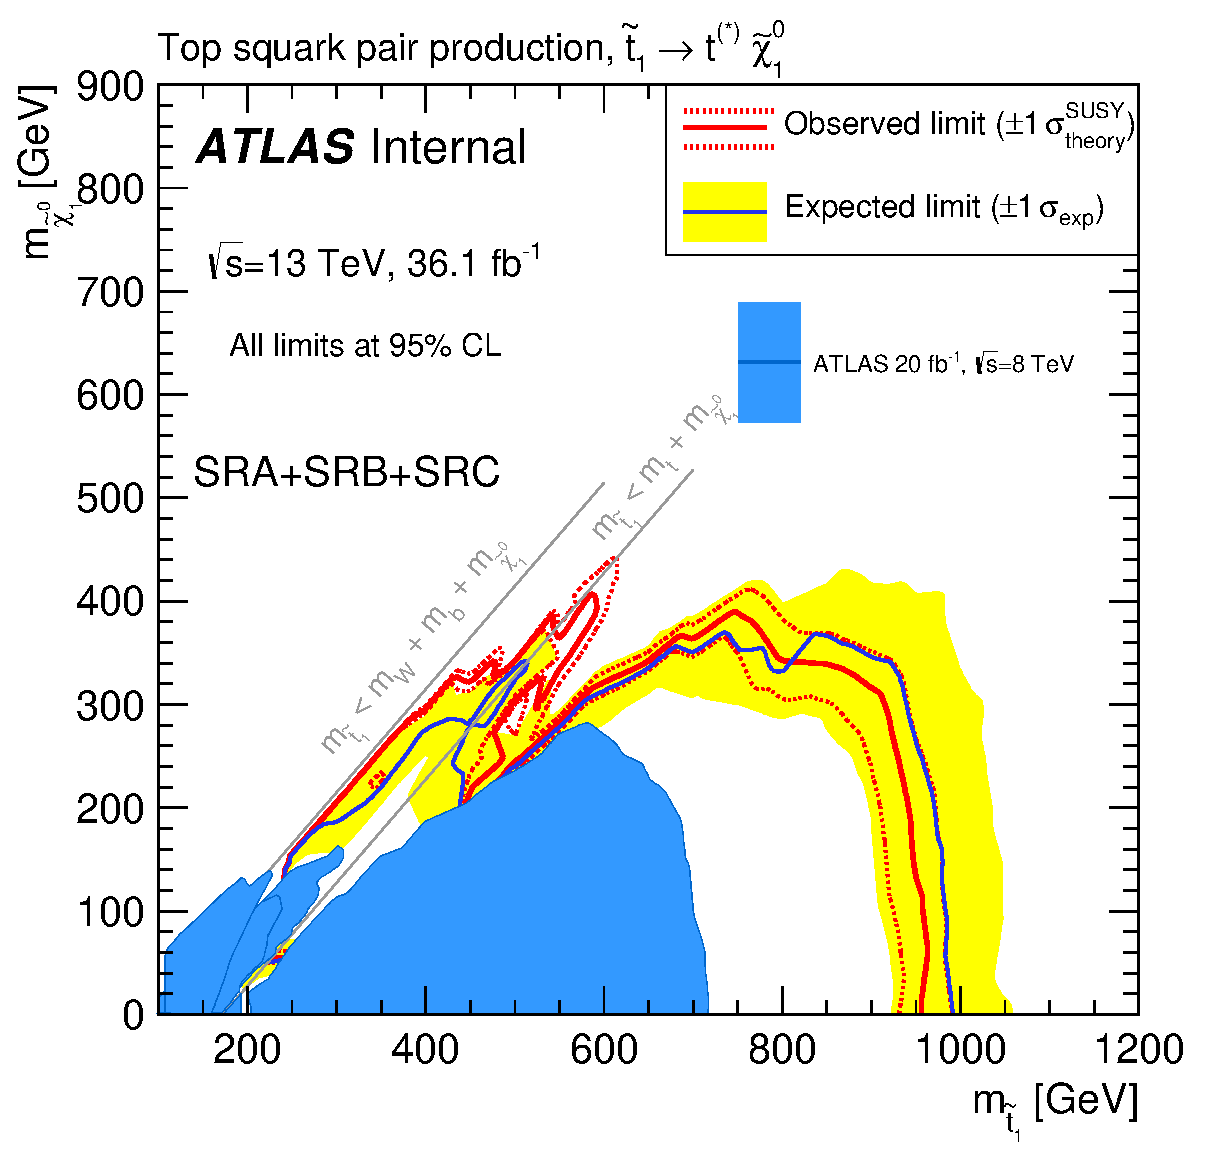
\includegraphics[width=0.85\textwidth]{figures/fit/atlascls_m0m12_wband1_showcms0_StopZL2016_SRABC_Tt_directTTplusbWN_all_Output_fixSigXSecNominal_hypotest__1_harvest_list.eps}
		\caption[95\% confidence limit curves in the stop, neutralino mass parameter space for the compressed stop analysis and the bulk region stop 0L analysis]{
		95\% confidence limit curves in the stop, neutralino mass parameter space for the compressed stop analysis (SRC) and the bulk region stop 0L analysis (SRA+SRB).The solid red (black) line correspond to the 95\% confidence observed (expected) limit curve from all three analysis combined. All regions below the curve has been excluded to the 95\% confidence level.  The dashed red line is the 95\% confidence limit on stop signal with a $1\sigma$ increase/decrease in signal production cross section.  The shaded yellow region correspond to the $1\sigma$ variation on the expected limit curve.  The variation on the expected limit curve is derived by fitting independent toy experiments and deriving an envelope of confidence limits.  95\% confidence limits from previous ATLAS stop searches using the 8 TeV collision dataset are shown as the shaded blue region for comparison.  The SRA and SRB analyses target high stop masses with large $\Delta m$ and medium amount of $\Delta m$.  Together these two analyses are sensitive to stop masses up $\sim900-1000 \gev$ if the neutralino mass is below $\sim350 \gev$. SRC correspond to the compressed region analysis and adds sensitivity to the $\Delta m = m_{t}$ diagonal region where SRA, SRB and the 8 TeV ATLAS stop searches lack sensitivity.   }
		\label{figure.exclusion.SRABC}
	\end{center}
\end{figure}

\indent Figure \ref{figure.exclusion.SRABCD_dm1} show how the exclusion limit changes for stops with different branching fractions to the $\stop \rightarrow t+\ninoone$ decay channel and the $\stop \rightarrow b+\chinoonepm$ decay channel.  As the $\stop \rightarrow t+\ninoone$ branching fraction decreases, the $\stop \rightarrow b+\chinoonepm$ branching fraction increases with total branching ratio of the two channels summing to 100\%.  Sensitivity from another signal region (SRD) that directly targets the mixed decay channel is combined with the compressed analysis (SRC) and the bulk region analyses (SRA+SRB).  Detailed documentation on the mixed decay analysis can also be found in reference [\cite{stop0LCONF}].  Again the compressed analysis is responsible for the exclusion of stop parameter space along the $\Delta m = m_{t}$ diagonal line when branching fraction to $\stop \rightarrow t+\ninoone$ is high. \\

\begin{figure}[h!]
	\begin{center}
		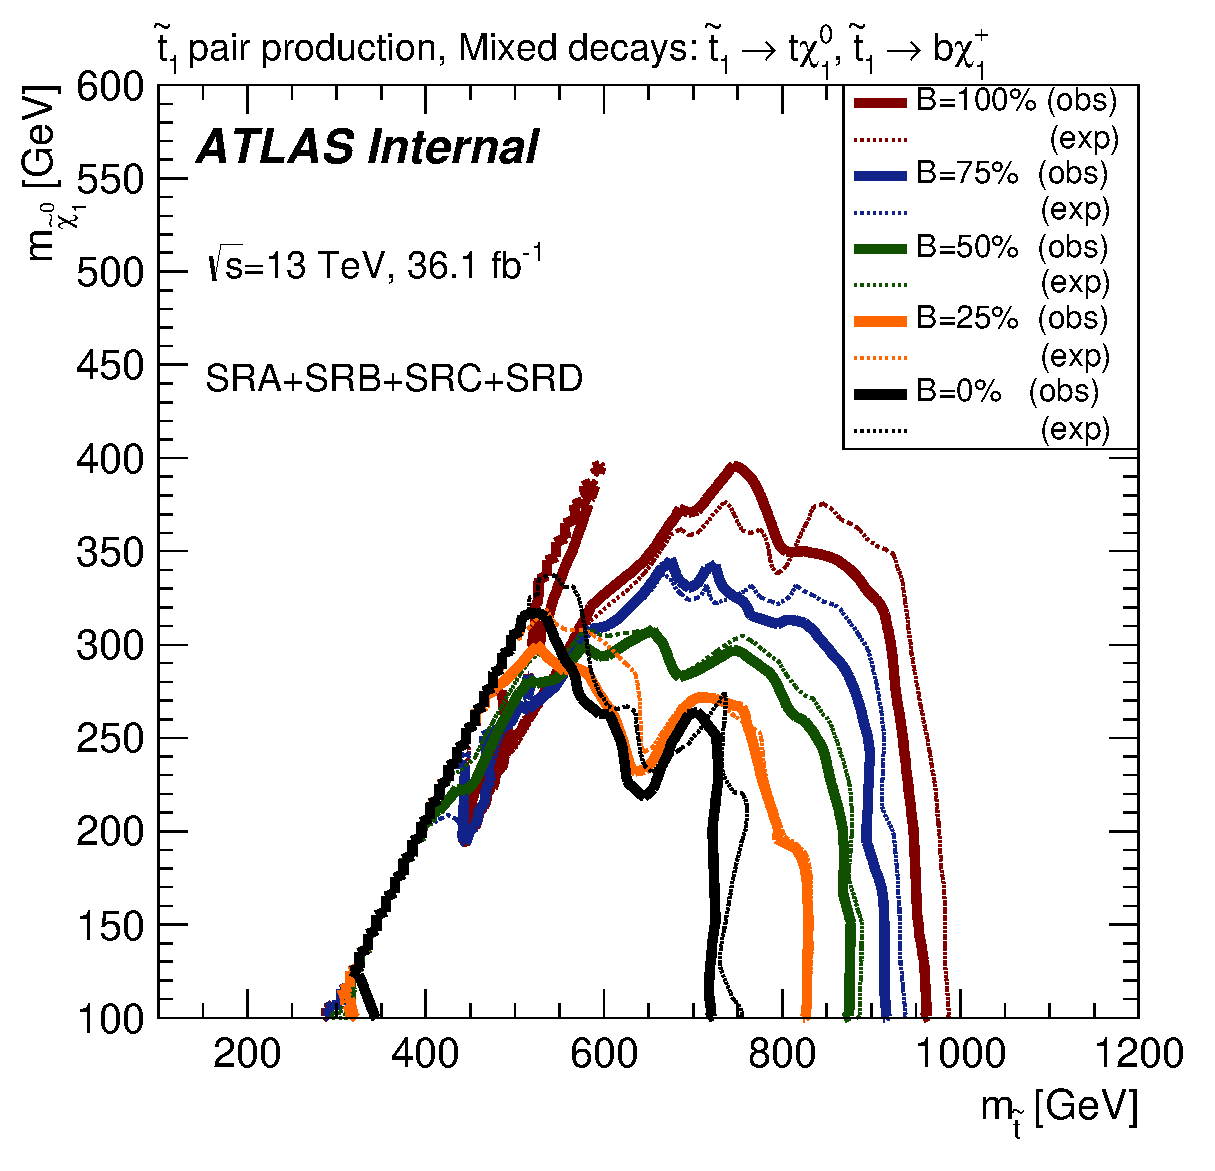
\includegraphics[width=0.85\textwidth]{figures/fit//SRABCD_mixed_dm1.eps}
		\caption[Observed 95\% confidence limits in the stop, neutralino mass plane for different branching ratios between the $\stop\ra t\ninoone$ decay channel
                  and the $\stop\ra b\chinoonepm$ channel]{
		95\% confidence limit curves in the stop, neutralino mass plane for different branching ratios between the $\stop\ra t\ninoone$ decay channel
                  and the $\stop\ra b\chinoonepm\ra b W^{(*)}\ninoone$ decay channel. 
                  The different curves correspond to different branching ratio values of the
                  $\stop\ra t\ninoone$ decay channel: 0\%, 25\%, 50\%, 75\% and 100\%.  
                   $m(\chinoonepm)$ is assumed to be $m(\ninoone)+1 GeV$ which is a good assumption for some
                   wino and Higgsino LSP SUSY models.  The chargino and neutralino LSP should has a small mass
                   difference if the LSP is a wino or a Higgsino because of the SU(2) symmetry in the weak interaction.
                  The results are based on a combination of the compressed stop analysis (SRC) targeting $\stop\ra t\ninoone$ with $\Delta m = m_{\stop} - m_{\ninoone} = m_{t}$, the bulk region stop zero-lepton search (SRA+SRB) targeting $\stop\ra t\ninoone$ with $\Delta m >> m_{t}$ region, and the mixed decay stop search (SRD) targeting stops that decays via both the $\stop\ra t\ninoone$ and $\stop\ra b\chinoonepm$ decay channels.  The we combine the different analysis by selecting for the best
                  expected $CL_s$ value at each stop and neutralino mass for the specific branching ratio. 
                   The compressed analysis SRC adds sensitivity to the $\Delta m = m_t$ line when the branching fraction is mostly to $\stop\ra t\ninoone$.}
		\label{figure.exclusion.SRABCD_dm1}
	\end{center}
\end{figure}